\documentclass[11pt]{article}

\usepackage[preprint]{acl}

\usepackage{times}
\usepackage{latexsym}
\usepackage[T1]{fontenc}
\usepackage[utf8]{inputenc}
\usepackage{microtype}
\usepackage{inconsolata}
\usepackage{xurl}
\usepackage{graphicx}
\usepackage{amsmath}
\usepackage{booktabs}
\usepackage{array}

\title{ZeroShotVDR: Query-Adaptive Two-Stage Retrieval for Zero-Shot Visual Document Retrieval}

\author{ZeroShotVDR Project Team \\
  Nanjing University \\
  \texttt{course project report}}

\begin{document}
\maketitle

\begin{abstract}
Zero-shot visual document retrieval requires finding evidence pages for a text query in visually rich long documents without task-specific training. OCR-only pipelines can miss layout, chart, figure, and table evidence, while OCR-free late-interaction retrievers such as ColPali provide strong page-level matching at a nontrivial scoring cost. This report presents ZeroShotVDR, a ColPali-based retrieval system for MMLongBench DocumentQA. We first build a stable baseline with source-image-derived page identities and a valid-only evaluation protocol that removes queries with unusable page supervision. We then propose a query-adaptive two-stage retrieval pipeline: mean-pooled page vectors provide coarse retrieval within the query-specific candidate universe, an adaptive selector chooses a bounded reranking set, neighbor expansion adds adjacent pages around high-ranked seeds, and full MaxSim reranking produces the final ranking. On 14,385 valid DocumentQA queries, the final Adaptive + Neighbor + MeanPoolCache system reaches Recall@10 = 0.8523 and nDCG@10 = 0.6325, compared with 0.8517 and 0.6325 for the full MaxSim baseline, while reducing average latency from 0.0716 to 0.0600 seconds/query and P95 latency from 0.1384 to 0.0858 seconds/query. The strongest gains appear on long-context SlideVQA slices, showing that adaptive coarse-to-fine retrieval improves the quality-efficiency trade-off for large candidate sets.
\end{abstract}

\section{Introduction}

Large document collections increasingly contain visually rich pages: tables, charts, figures, presentation slides, multi-column layouts, and cross-region references. For page-level document retrieval, the relevant evidence is often not captured by plain OCR text alone. A chart may answer a query through axis labels and plotted values; a slide may express the needed relation through layout and figure captions; a report page may combine text, tables, and visual grouping. These cases motivate visual document retrieval (VDR), where a system receives a text query and ranks document pages directly from page images.

The course task is therefore not only to obtain high retrieval accuracy, but also to consider the cost of indexing, storage, and inference. This is a practical constraint for visual retrieval. Page images are much heavier than text passages, and patch-level visual embeddings are much larger than sparse text-index entries. A system that scores every page with a fine-grained interaction function may be accurate on a small document, yet become unnecessarily expensive when each query brings dozens or hundreds of candidate pages. The central question of this report is how to retain the strength of ColPali-style visual matching while reducing avoidable full-interaction computation.

This project targets zero-shot VDR. The system does not train on MMLongBench; instead, it uses ColPali-v1.3 as an OCR-free visual retriever. ColPali encodes each page as patch-level visual-language embeddings and scores a query through late interaction, following the MaxSim idea popularized by ColBERT \citep{khattab2020colbert}. This design preserves fine-grained visual evidence and provides a strong baseline for page retrieval \citep{faysse2024colpali}. Its cost, however, grows with the number of candidate pages and with the number of page patches scored by MaxSim. In long-context settings, this cost becomes more visible, and visually similar neighboring pages can also make the ranking less robust.

We evaluate on the DocumentQA subset of MMLongBench \citep{wang2025mmlongbench,mmlongbenchdataset}, which provides page-level answer annotations through \texttt{ans\_page\_list}. The project uses three DocumentQA subtasks: \texttt{longdocurl}, \texttt{mmlongdoc}, and \texttt{slidevqa}, across length buckets K4, K8, K16, K32, K64, and K128. The data format naturally defines a query-specific page candidate universe through each sample's \texttt{page\_list}. Our evaluation therefore studies query-scoped candidate retrieval rather than global corpus retrieval. This distinction is important: the reported numbers measure how well the system ranks pages within the provided long-document context, not whether it can first identify the correct document from a global collection.

The final system combines two stages. The first stage uses a mean-pooled view of page patch embeddings to cheaply rank candidate pages. The second stage applies full ColPali MaxSim only to a smaller candidate set. Instead of choosing a fixed top-$N$, the system selects a query-adaptive number of candidates from the coarse score distribution, then expands around top seed pages with a small neighbor window. A precomputed mean-pool cache further removes repeated coarse-stage computation. This design is motivated by Phase 3 failure analysis: the hardest cases concentrate in large candidate sets and in neighboring or visually repetitive pages, especially long SlideVQA slices.

The project went through two engineering corrections before this method could be evaluated fairly. First, stable page identity had to be reconstructed from source image paths instead of sample-local enumeration. Without this correction, a predicted page and a ground-truth page could refer to incompatible page identities even if they had similar local indices. Second, the evaluation had to distinguish real retrieval failures from queries whose page-level supervision was unusable. These corrections are not the main algorithmic contribution, but they are essential for trustworthy comparison.

The contributions are:
\begin{itemize}
    \item We build a stable ColPali-based page retrieval baseline for MMLongBench DocumentQA, including source-image-derived page identity reconstruction and a valid-only evaluation protocol over 14,385 usable queries.
    \item We propose a query-adaptive two-stage retrieval method that combines mean-pool coarse retrieval, adaptive candidate sizing, neighbor-aware expansion, and full MaxSim reranking.
    \item We show that the final system preserves retrieval quality while improving efficiency, with the clearest quality-efficiency gains on long-context SlideVQA and K128 candidate buckets.
\end{itemize}

\section{Related Work}

\paragraph{OCR-free visual document retrieval.}
Traditional document retrieval pipelines often convert pages into text with OCR and then index the extracted text. Such pipelines are effective when the answer evidence is mostly textual, but they can lose layout, visual grouping, figure content, and table structure. ColPali instead embeds rendered document pages directly with a vision-language model and performs page retrieval without a separate OCR stage \citep{faysse2024colpali,colpalimodel}. Our project uses ColPali as the main baseline and studies how to make its page-level late-interaction scoring more efficient under long candidate sets.

The focus of this report differs from work that attempts to replace visual retrieval with text retrieval or OCR post-processing. We assume that page images remain the retrieval unit and that ColPali's patch-level evidence is valuable. The improvement is therefore not a new document encoder, but a reranking policy and cache design around an existing strong visual retriever.

\paragraph{Late interaction retrieval.}
Late interaction keeps token-level or patch-level representations until scoring time. ColBERT introduced this design for text passage retrieval: query token vectors interact with document token vectors through MaxSim, preserving fine-grained matching while allowing efficient retrieval compared with full cross-encoders \citep{khattab2020colbert}. ColPali transfers this idea to visual document pages by matching query token embeddings against page patch embeddings. The advantage is expressive matching; the limitation is that each candidate page still requires many vector comparisons. ZeroShotVDR keeps full MaxSim as the final scoring function but tries to reduce how often it is applied.

This choice is conservative. The final method keeps the original patch-level evidence intact and uses a cheaper page-level view only as a candidate controller. This fits the observed failure cases, where fine-grained visual evidence is still important even though full MaxSim over every candidate is expensive.

\paragraph{Long-context vision-language evaluation.}
MMLongBench evaluates long-context vision-language models across several task families and standardized context lengths \citep{wang2025mmlongbench}. DocumentQA is the most direct fit for this project because its \texttt{ans\_page\_list} annotations can be interpreted as page-level relevance labels. The benchmark also exposes the difficulty of long candidate sets: as the candidate universe grows, retrieval must distinguish relevant pages from many visually similar distractors.

\section{Task and Method}

\subsection{Task Definition and Protocol}

For each query $q$, the input contains a query-specific candidate page set $C(q)=\{p_1,\ldots,p_n\}$ derived from the sample's \texttt{page\_list}. The task is to rank pages in $C(q)$ so that pages in the answer page set $G(q)$, derived from \texttt{ans\_page\_list}, appear as high as possible. The main evaluation uses Recall@k, Precision@k, MRR, and nDCG@k.

The main protocol uses only queries with usable page-level supervision. The raw full run contains 15,577 queries, but 1,192 have empty, invalid, or out-of-range answer page annotations. These cases are excluded from the main comparison because an empty relevant set would otherwise make recall and MRR misleading. The final main set contains 14,385 valid queries. Full-query results are retained only as appendix-level disclosure.

A second protocol decision concerns page identity. In early experiments, page IDs built from sample-local document names and page enumeration were not stable across long-context samples. The stable implementation reconstructs page identity from source image paths and uses a normalized format that includes task family, subtask, length bucket, source document ID, and source page index. Each query also carries \texttt{candidate\_page\_ids}, which fixes the query-scoped candidate universe.

The protocol can be summarized as follows. For a query with valid annotations, all methods receive the same $C(q)$ and the same ground-truth set $G(q)$. The baseline ranks all pages in $C(q)$ with full MaxSim. Phase 4 methods may internally choose a smaller reranking set, but they are not allowed to use pages outside $C(q)$ unless an explicit global-retrieval experiment is configured. This keeps all comparisons aligned with the DocumentQA sample structure.

\subsection{Stable ColPali Baseline}

The baseline contains five layers: a data adapter for MMLongBench DocumentQA, an indexing layer that stores per-page embeddings, a retrieval layer, an evaluation layer, and configuration support. Each page image is encoded by ColPali-v1.3 into a matrix of patch embeddings. Each query is encoded into token embeddings. Given L2-normalized query vectors $\hat{q}_i$ and page patch vectors $\hat{p}_j$, the baseline score is
\begin{equation}
S_{\mathrm{max}}(Q,P)=
\sum_{i=1}^{|Q|}\max_{1 \leq j \leq |P|}
\langle \hat{q}_i, \hat{p}_j\rangle .
\end{equation}
The baseline applies this full MaxSim score to every page in $C(q)$ and returns the top-ranked pages. Because $C(q)$ is query-scoped, the average baseline candidate universe over valid queries is 32.7 pages, while long buckets such as K128 are much larger.

The index is stored as independent page files rather than one monolithic tensor. This choice makes the implementation slower to describe but improves page-level traceability: pages can be loaded by stable ID, retrieval outputs can be audited against source images, and evaluation can use the same page identity contract throughout the pipeline. The final stable full run uses an index size of about 88.6 GB, so the implemented efficiency gain should be understood as an inference-time reranking improvement rather than a replacement for the full patch index.

\subsection{Query-Adaptive Two-Stage Retrieval}

The proposed method keeps the baseline's final scorer but changes how candidates reach it. Figure~\ref{fig:pipeline} summarizes the pipeline.

\begin{figure*}[t]
\centering
\setlength{\fboxsep}{6pt}
\fbox{
\begin{minipage}{0.94\linewidth}
\centering
\textbf{Query-specific universe} $\rightarrow$
\textbf{mean-pool coarse ranking} $\rightarrow$
\textbf{adaptive top-$N$ selection} $\rightarrow$
\textbf{neighbor expansion} $\rightarrow$
\textbf{full MaxSim reranking} $\rightarrow$
\textbf{top-$k$ pages}

\vspace{0.6em}
\small
The coarse stage ranks only pages in \texttt{candidate\_page\_ids}. The final stage keeps ColPali's full patch-level MaxSim, but applies it to a reduced and neighbor-aware candidate set. A mean-pool cache precomputes page vectors used by the coarse stage.
\end{minipage}}
\caption{ZeroShotVDR retrieval pipeline.}
\label{fig:pipeline}
\end{figure*}

\paragraph{Mean-pool coarse retrieval.}
For each page $P$, the system computes a single vector by averaging patch embeddings:
\begin{equation}
\bar{p}=\frac{1}{|P|}\sum_{j=1}^{|P|}\hat{p}_j .
\end{equation}
The query also receives a mean vector $\bar{q}$. Coarse ranking uses the dot product between normalized mean vectors. This representation is much cheaper than full MaxSim because each page contributes one vector instead of all patches.

\paragraph{Adaptive candidate selection.}
A fixed top-$N$ coarse cutoff is simple but brittle. Small candidate universes do not need aggressive pruning, while flat coarse score distributions may require more candidates to avoid dropping relevant evidence. The adaptive selector uses a bounded candidate count with minimum 32, maximum 128, base ratio 0.2, and a flat-score margin of 0.035. The selected count is clipped by the available universe size. This makes the reranking budget depend on each query's candidate set and score shape rather than on a single global constant.

In practical terms, the adaptive rule behaves like a low-risk controller. When the universe is small, it often keeps all pages and therefore matches the baseline candidate set. When the universe is large and the coarse ranking is decisive, it keeps a much smaller reranking set. When scores are flatter, it can retain more pages up to the maximum bound. This explains why the overall average rerank count falls to about 19.8 for the final method, while the K128 bucket still keeps about 34.8 pages on average.

\paragraph{Neighbor expansion.}
DocumentQA evidence often spans adjacent pages, and baseline errors include neighbor-page confusion. After adaptive selection, the system expands around the top coarse seeds by adding pages within a one-page window when those pages are present in the query-specific universe. The full run uses eight seed pages. This expansion is deliberately small: it recovers likely adjacent evidence without returning to full-universe reranking.

Neighbor expansion is especially natural for slide decks and long reports. If a coarse stage identifies a page near the answer, the immediately previous or next page often shares section context or contains the continuation of a visual explanation. However, expanding all selected pages would quickly destroy the computational benefit. The implementation therefore expands only around the top seed pages.

\paragraph{Mean-pool cache.}
The mean-pooled page view can be computed on the fly, but repeated full runs benefit from a cache. The final system uses a MeanPoolCache with 87,090 cached page vectors, embedding dimension 128, and float16 storage. Its directory size is about 26 MB, compared with about 88.6 GB for the original patch index. The cache changes coarse-stage efficiency, not ranking quality, because the same mean vectors are used.

\subsection{Expected Complexity Benefit}

Let $m$ be the number of query token embeddings, $r$ the number of patch embeddings per page, $d$ the embedding dimension, and $n=|C(q)|$. Full baseline scoring scales as $O(nmrd)$ for each query. The proposed method adds an $O(nd)$ coarse pass but reduces full MaxSim to $a(q)$ candidates, where $a(q) \leq n$ is the adaptive expanded size. The method is therefore most useful when $n$ is large, which matches the observed long-context failure slices.

\section{Experimental Setup}

\subsection{Dataset}

Experiments use MMLongBench DocumentQA. The evaluated subtasks are \texttt{longdocurl}, \texttt{mmlongdoc}, and \texttt{slidevqa}. Each subtask is evaluated across K4, K8, K16, K32, K64, and K128 length buckets. The main valid-only set contains 14,385 queries. The stable baseline full run indexes 87,922 pages and produces a patch index of about 88.6 GB.

\begin{table*}[t]
\centering
\small
\begin{tabular}{lrrrrrrr}
\toprule
Subtask & K4 & K8 & K16 & K32 & K64 & K128 & Total \\
\midrule
\texttt{longdocurl} & 84 & 771 & 914 & 1060 & 1141 & 1153 & 5123 \\
\texttt{mmlongdoc} & 53 & 410 & 591 & 663 & 707 & 726 & 3150 \\
\texttt{slidevqa} & 930 & 1000 & 1041 & 1047 & 1047 & 1047 & 6112 \\
\midrule
Total & 1067 & 2181 & 2546 & 2770 & 2895 & 2926 & 14385 \\
\bottomrule
\end{tabular}
\caption{Valid-only query counts by subtask and length bucket.}
\label{tab:scope}
\end{table*}

Table~\ref{tab:scope} shows the valid-only evaluation scope. The distribution is not uniform: SlideVQA contributes many more K4 examples than the other subtasks, while all three subtasks contribute to K128. This is why the report presents both overall metrics and slice-level analysis. Overall numbers are useful for the final method comparison, but they can hide subtask-specific behavior.

\subsection{Metrics}

Quality is measured by Recall@k, Precision@k, MRR, and nDCG@k for $k \in \{1,3,5,10\}$. The main tables focus on Recall@10, Precision@10, MRR, and nDCG@10 because top-10 page retrieval is the target setting. Efficiency is measured by average latency, P95 latency, and average number of full MaxSim rerank candidates.

Recall@k measures the fraction of relevant pages recovered in the top $k$, while Precision@k measures how many of the top $k$ returned pages are relevant. MRR reflects how early the first relevant page appears, and nDCG@k rewards relevant pages appearing near the top while supporting multiple relevant pages. In this task, Recall@10 and nDCG@10 are the most informative main metrics because many queries have one or a few answer pages and the downstream use case expects a short list of evidence pages.

\subsection{Compared Systems}

The comparison includes the Phase 3 Full MaxSim baseline, fixed two-stage variants with top-32, top-64, and top-128 coarse candidates, Adaptive + MaxSim, Adaptive + Neighbor + MaxSim, and cache variants for Fixed Top-64, Adaptive, and Adaptive + Neighbor. The final recommended system is Adaptive + Neighbor + Cache.

\subsection{Implementation}

The model is ColPali-v1.3. Experiments were run on Ubuntu with two NVIDIA RTX 3090 GPUs with 24 GB memory each. Indexing and retrieval are separated. The index stores each page independently, which supports page-level loading, stable evaluation, and per-query trace analysis. The main entry points are the unified command-line script and Phase 3/Phase 4 evaluation scripts in the project repository.

All Phase 4 runs produce a summary file, overall metrics, metrics by subtask and length, bucket metrics, slice metrics, and per-query traces. The final run uses \texttt{adaptive\_neighbors} with mean-pool cache enabled. The mean-pool cache was built in batches after an earlier full-cache construction attempted to materialize too many page vectors at once. The final batched cache construction completed at full scale and is used for the recommended system.

\section{Results}

\subsection{Main Ablation}

Table~\ref{tab:main} reports the main valid-only ablation. The full MaxSim baseline obtains Recall@10 = 0.8517 and nDCG@10 = 0.6325. The final no-cache Adaptive + Neighbor variant slightly improves Recall@10 to 0.8523 while keeping nDCG@10 essentially unchanged.

\begin{table*}[t]
\centering
\small
\begin{tabular}{lrrrrrrr}
\toprule
Method & R@10 & P@10 & MRR & nDCG@10 & Avg Lat. & P95 Lat. & Rerank \\
\midrule
Phase 3 Full MaxSim & 0.8517 & 0.1218 & 0.5838 & 0.6325 & 0.0716 & 0.1384 & 32.7 \\
Fixed Top-32 + MaxSim & 0.8482 & 0.1211 & 0.5828 & 0.6308 & 0.0794 & 0.1434 & 19.0 \\
Fixed Top-64 + MaxSim & 0.8513 & 0.1217 & 0.5839 & 0.6325 & 0.0889 & 0.1800 & 26.8 \\
Fixed Top-128 + MaxSim & 0.8517 & 0.1218 & 0.5839 & 0.6326 & 0.0907 & 0.1989 & 32.2 \\
Adaptive + MaxSim & 0.8482 & 0.1211 & 0.5828 & 0.6308 & 0.0790 & 0.1417 & 19.0 \\
Adaptive + Neighbor + MaxSim & \textbf{0.8523} & 0.1217 & 0.5838 & 0.6325 & 0.0796 & 0.1437 & 19.8 \\
\bottomrule
\end{tabular}
\caption{Main valid-only ablation over 14,385 queries. Latencies are seconds/query. Rerank is the average number of pages scored by full MaxSim.}
\label{tab:main}
\end{table*}

The fixed top-$N$ variants show why adaptation and neighbor expansion are needed. Top-32 and Adaptive both reduce rerank candidates to 19.0 but lose a small amount of quality. Top-128 recovers baseline quality, but it is slower than the baseline because it adds a coarse pass while still reranking almost the same number of pages. Neighbor expansion is the main quality recovery mechanism: it keeps the small reranking set but restores Recall@10 above the baseline.

The main table also shows that Precision@10 changes very little across methods. This is expected because the average number of relevant answer pages is small and all systems return ten pages. Most quality differences appear through recall and ranking-sensitive nDCG rather than large changes in top-10 precision. The important result is therefore not a large absolute quality improvement, but the ability to preserve the baseline quality while reducing the expensive part of inference.

\begin{figure*}[t]
\centering
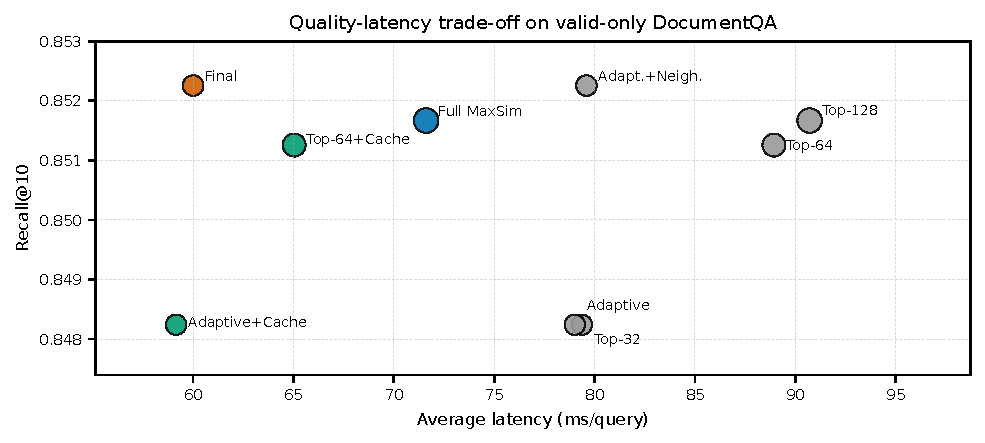
\includegraphics[width=0.88\linewidth]{figures/quality_latency_tradeoff.pdf}
\caption{Quality-latency trade-off across the main baseline, ablations, and cache variants. Marker size reflects the average number of pages reranked with full MaxSim. The final method is the fastest high-recall point.}
\label{fig:quality-latency}
\end{figure*}

\subsection{Effect of Mean-Pool Cache}

Table~\ref{tab:cache} isolates the cache effect. The cache preserves the exact quality of each corresponding no-cache method and reduces latency. For the recommended Adaptive + Neighbor method, average latency drops from 0.0796 to 0.0600 seconds/query, and P95 latency drops from 0.1437 to 0.0858 seconds/query. Compared with the Phase 3 baseline, the final system keeps nDCG@10 unchanged, improves Recall@10 by 0.0006, and reduces P95 latency by 38.0\%.

\begin{table*}[t]
\centering
\small
\begin{tabular}{lrrrr}
\toprule
Method & R@10 & nDCG@10 & Avg Lat. & P95 Lat. \\
\midrule
Fixed Top-64 & 0.8513 & 0.6325 & 0.0889 & 0.1800 \\
Fixed Top-64 + Cache & 0.8513 & 0.6325 & 0.0650 & 0.1178 \\
Adaptive & 0.8482 & 0.6308 & 0.0790 & 0.1417 \\
Adaptive + Cache & 0.8482 & 0.6308 & 0.0592 & 0.0847 \\
Adaptive + Neighbor & 0.8523 & 0.6325 & 0.0796 & 0.1437 \\
Adaptive + Neighbor + Cache & \textbf{0.8523} & \textbf{0.6325} & \textbf{0.0600} & \textbf{0.0858} \\
\bottomrule
\end{tabular}
\caption{Cache comparison. Latencies are seconds/query.}
\label{tab:cache}
\end{table*}

\subsection{Long Candidate Buckets}

The main efficiency gain appears when the candidate universe is large. Table~\ref{tab:k128} shows the K128 universe bucket. The final method reduces average rerank candidates from 81.1 to 34.8 and P95 latency from 189.2 ms to 97.4 ms. It also improves Recall@10 from 0.6818 to 0.6882 and nDCG@10 from 0.3902 to 0.3916.

This bucket-level result is more informative than the overall average latency alone. In short contexts, the baseline is already cheap because there are only a few pages to score. In K128, the baseline must run full MaxSim over many more pages, and the two-stage design has room to remove work. This is the setting for which the method was designed.

\begin{figure*}[t]
\centering
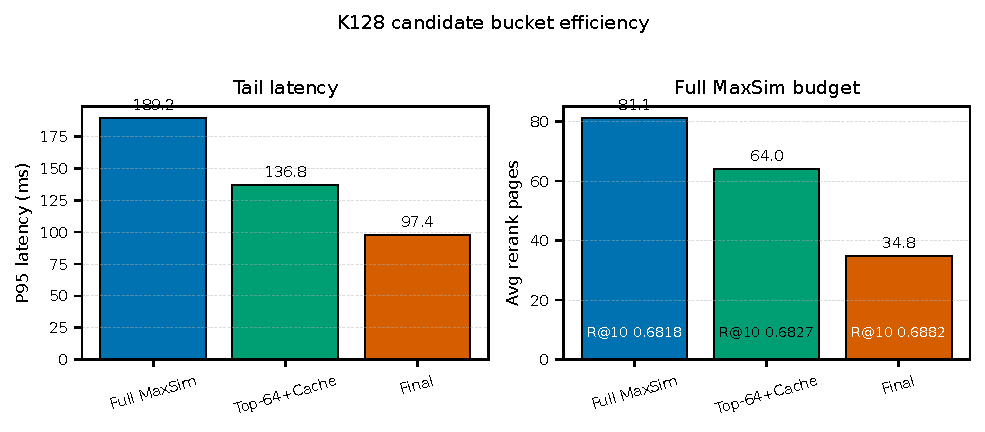
\includegraphics[width=0.86\linewidth]{figures/k128_efficiency.pdf}
\caption{Efficiency comparison on the K128 candidate bucket. The final method substantially reduces both tail latency and the full MaxSim reranking budget while slightly improving Recall@10.}
\label{fig:k128-efficiency}
\end{figure*}

\begin{table*}[t]
\centering
\small
\begin{tabular}{lrrrrr}
\toprule
Method & R@10 & nDCG@10 & Avg ms & P95 ms & Rerank \\
\midrule
Full MaxSim & 0.6818 & 0.3902 & 109.6 & 189.2 & 81.1 \\
Fixed Top-64 + Cache & 0.6827 & 0.3902 & 96.4 & 136.8 & 64.0 \\
Adaptive + Neighbor + Cache & \textbf{0.6882} & \textbf{0.3916} & \textbf{71.5} & \textbf{97.4} & \textbf{34.8} \\
\bottomrule
\end{tabular}
\caption{K128 candidate-bucket results. Latencies are milliseconds/query.}
\label{tab:k128}
\end{table*}

\subsection{Slice-Level Analysis}

Table~\ref{tab:slices} compares the final method against the baseline on the five key slices identified in failure analysis. The strongest quality gains are on \texttt{slidevqa/K128} and \texttt{slidevqa/K64}. These slices have many visually repetitive slide pages, so mean-pool coarse ranking plus neighbor expansion can remove many distractors while preserving adjacent evidence. The method is not uniformly better: \texttt{mmlongdoc/K128} and \texttt{longdocurl/K128} lose a small amount of quality while gaining latency and reranking efficiency.

This is the main empirical nuance of the project. If the report only stated the overall Recall@10 improvement, it would overstate the method. The realistic conclusion is that the method improves the global quality-efficiency trade-off and helps the hardest SlideVQA slices, but it can trade a small amount of quality for efficiency on some long-document slices. This trade-off is acceptable for the project goal because the advanced task allows either better retrieval performance or lower computation/storage cost under comparable quality.

\begin{figure*}[t]
\centering
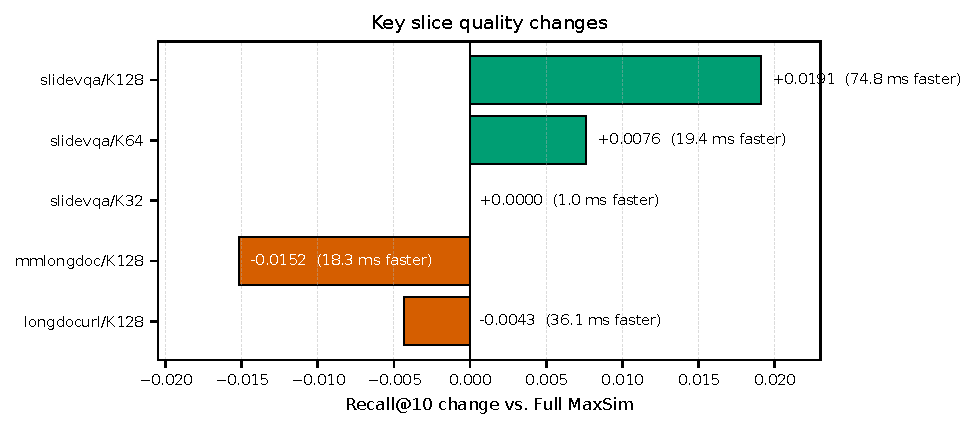
\includegraphics[width=0.82\linewidth]{figures/slice_recall_delta.pdf}
\caption{Recall@10 changes on the five key slices used in failure analysis. Positive gains concentrate on long SlideVQA slices, while long document slices show small quality regressions but lower latency.}
\label{fig:slice-delta}
\end{figure*}

\begin{table*}[t]
\centering
\scriptsize
\begin{tabular}{lrrrrrrrr}
\toprule
Slice & Base R@10 & Final R@10 & $\Delta$R & Base nDCG & Final nDCG & $\Delta$nDCG & Base ms & Final ms \\
\midrule
\texttt{slidevqa/K128} & 0.5597 & 0.5788 & +0.0191 & 0.2528 & 0.2597 & +0.0069 & 143.2 & 68.4 \\
\texttt{slidevqa/K64} & 0.6036 & 0.6113 & +0.0076 & 0.2736 & 0.2754 & +0.0018 & 89.0 & 69.6 \\
\texttt{slidevqa/K32} & 0.6533 & 0.6533 & +0.0000 & 0.2956 & 0.2956 & +0.0000 & 67.1 & 66.1 \\
\texttt{mmlongdoc/K128} & 0.9022 & 0.8871 & -0.0152 & 0.6887 & 0.6809 & -0.0078 & 88.3 & 70.0 \\
\texttt{longdocurl/K128} & 0.9584 & 0.9540 & -0.0043 & 0.7597 & 0.7563 & -0.0035 & 113.5 & 77.4 \\
\bottomrule
\end{tabular}
\caption{Key slice comparison between Phase 3 Full MaxSim and final Adaptive + Neighbor + Cache.}
\label{tab:slices}
\end{table*}

\section{Discussion}

\subsection{Why Adaptive Coarse-to-Fine Helps}

The method helps when the cost and ambiguity of full-universe MaxSim are high. In small candidate sets, a coarse stage cannot remove much work. In long candidate sets, however, many pages can be eliminated with a cheap mean-pooled view. This explains the K128 bucket result and the SlideVQA improvements. Slide decks often contain repeated templates and neighboring pages from the same topic. Coarse ranking identifies plausible regions, and neighbor expansion adds adjacent pages that might contain partial or continuation evidence.

The mean-pooled representation is intentionally weak compared with MaxSim. It cannot replace token-patch late interaction because averaging removes spatial and token-level detail. Its role is instead to estimate which pages are plausible enough to deserve the expensive scorer. This separation is why the method can gain efficiency without redesigning the underlying model.

\subsection{Where the Trade-off Appears}

The final system does not dominate every slice. On \texttt{mmlongdoc/K128}, Recall@10 drops from 0.9022 to 0.8871. On \texttt{longdocurl/K128}, the drop is smaller, from 0.9584 to 0.9540. These cases suggest that some long reports and web documents contain dispersed fine-grained evidence that the mean-pooled coarse view may rank below the adaptive cutoff. Neighbor expansion reduces this risk but cannot fully replace full-universe MaxSim.

The trade-off also explains why fixed top-128 is not chosen as the final method. It is a safer candidate filter, but it loses most of the efficiency benefit and can even become slower than the baseline because the coarse stage is added on top of nearly full reranking. Adaptive selection is preferable because it changes the reranking budget only when the query and candidate set make pruning plausible.

\subsection{Failure Modes}

Phase 3 analysis identified three failure types: miss\_top10 under large candidate sets, partial recall for multi-page evidence, and neighbor-page confusion. The proposed method mainly addresses the first and third. It reduces the MaxSim budget on large candidate sets and explicitly includes adjacent pages around high-ranked coarse seeds. Multi-page partial recall remains harder because the current system ranks pages independently and does not model evidence aggregation across multiple pages.

This remaining failure mode is important when interpreting the results: the proposed method improves how individual pages are selected for reranking, but it does not explicitly aggregate evidence across multiple pages. The reported gains therefore come from better candidate control and neighbor recovery, not from cross-page reasoning.

\subsection{Limitations}

First, the evaluation is query-scoped candidate retrieval, not global corpus retrieval. This matches MMLongBench DocumentQA's sample structure, but the reported numbers should not be read as document-level retrieval from all pages in the corpus. Second, the mean-pool cache is compact, but the full patch index remains necessary for final MaxSim reranking; the storage footprint of the complete visual index is therefore still large. Third, the valid-only protocol is necessary for fair comparison, but it also means that 1,192 queries with unusable page-level supervision are excluded from the main table. Finally, latency numbers are hardware-dependent; the relative trends are more important than the absolute seconds/query on another machine.

Another limitation is that the adaptive rule is hand-designed. It is motivated by the score distribution and validated through ablations, but it is not learned. This is appropriate for the zero-shot course setting because it avoids training on the benchmark, while still making the reranking budget sensitive to query-level candidate structure.

\section{Conclusion}

ZeroShotVDR builds a stable ColPali-based page retrieval system for MMLongBench DocumentQA and improves it with a query-adaptive two-stage retrieval pipeline. The final Adaptive + Neighbor + MeanPoolCache method preserves the baseline's retrieval quality while reducing average and tail latency, especially on long candidate sets. The results support a conservative conclusion: adaptive coarse-to-fine reranking is an effective quality-efficiency improvement over full MaxSim for query-scoped zero-shot visual document retrieval, with the main remaining limitations being the query-scoped protocol, dependence on the full patch index for final reranking, and small quality regressions on some long-document slices.

\section*{Acknowledgments}

This report is based on the ZeroShotVDR course project implementation, project plan, milestone reports, and full evaluation outputs.

\bibliography{zeroshotvdrrefs}

\appendix

\section{Additional Results}

\begin{table}[h]
\centering
\small
\begin{tabular}{rrrrr}
\toprule
k & Recall & Precision & MRR & nDCG \\
\midrule
1 & 0.3342 & 0.4403 & 0.5838 & 0.4403 \\
3 & 0.6201 & 0.2853 & 0.5838 & 0.5435 \\
5 & 0.7250 & 0.2041 & 0.5838 & 0.5881 \\
10 & 0.8517 & 0.1218 & 0.5838 & 0.6325 \\
\bottomrule
\end{tabular}
\caption{Phase 3 Full MaxSim baseline on the 14,385-query valid-only subset.}
\label{tab:appendix-baseline}
\end{table}

\begin{table}[h]
\centering
\small
\begin{tabular}{rrrrr}
\toprule
k & Recall & Precision & MRR & nDCG \\
\midrule
1 & 0.3342 & 0.4403 & 0.5838 & 0.4403 \\
3 & 0.6198 & 0.2852 & 0.5838 & 0.5433 \\
5 & 0.7247 & 0.2040 & 0.5838 & 0.5879 \\
10 & 0.8523 & 0.1217 & 0.5838 & 0.6325 \\
\bottomrule
\end{tabular}
\caption{Final Adaptive + Neighbor + Cache system on the 14,385-query valid-only subset.}
\label{tab:appendix-final}
\end{table}

\section{Reproducibility Notes}

\begin{sloppypar}
\small
The main comparison uses:
\begin{itemize}
    \item Phase 3 baseline: \path{outputs/eval_reports/step3_docqa_full_dual3090_stable_page_ids/analysis/phase4_schema_valid_only/}.
    \item Final run: \path{outputs/eval_reports/phase4_adaptive_neighbors_cache_full_20260520/}.
    \item Mean-pool cache: \path{outputs/cache/mean_pool_full_20260520_rerun/}.
\end{itemize}

The final configuration uses method \path{adaptive_neighbors}, \texttt{min\_candidates=32}, \texttt{max\_candidates=128}, \texttt{base\_ratio=0.2}, \texttt{flat\_margin=0.035}, \texttt{neighbor\_window=1}, \texttt{neighbor\_seed\_n=8}, and \texttt{use\_mean\_pool\_cache=true}.
\end{sloppypar}

\end{document}
